%%%%%%%%%%%%%%%%%%%%%%%%%%%%%%%%%%%%%%%%%%%%%%%%%%%%%%%%%%%%%%%%%%%%%%%%%%%%%%%%

\section{The Central Limit Theorem}

The normal distribution is really important in statistical hypothesis testing (and in statistics generally), and its prominence arises from an important theorem called the \textbf{Central Limit Theorem}. 

The Central Limit Theorem states that \textbf{the sum of a large number of independent random variables will be normally distributed}. Importantly, \emph{it does not matter} what distribution(s) they are being pulled from. Also note that the fact that the sum is normally distributed also means the mean is normally distributed.

\begin{figure}[h]
\begin{center}
    \begin{subfigure}{0.4\textwidth}
    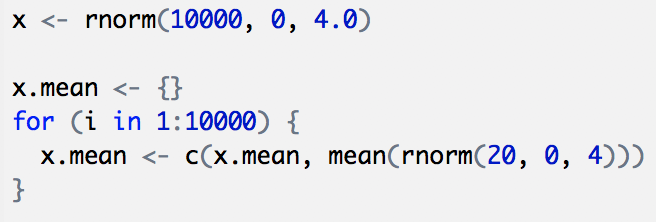
\includegraphics[width=\textwidth]{img/clt-rnorm-code.png}
    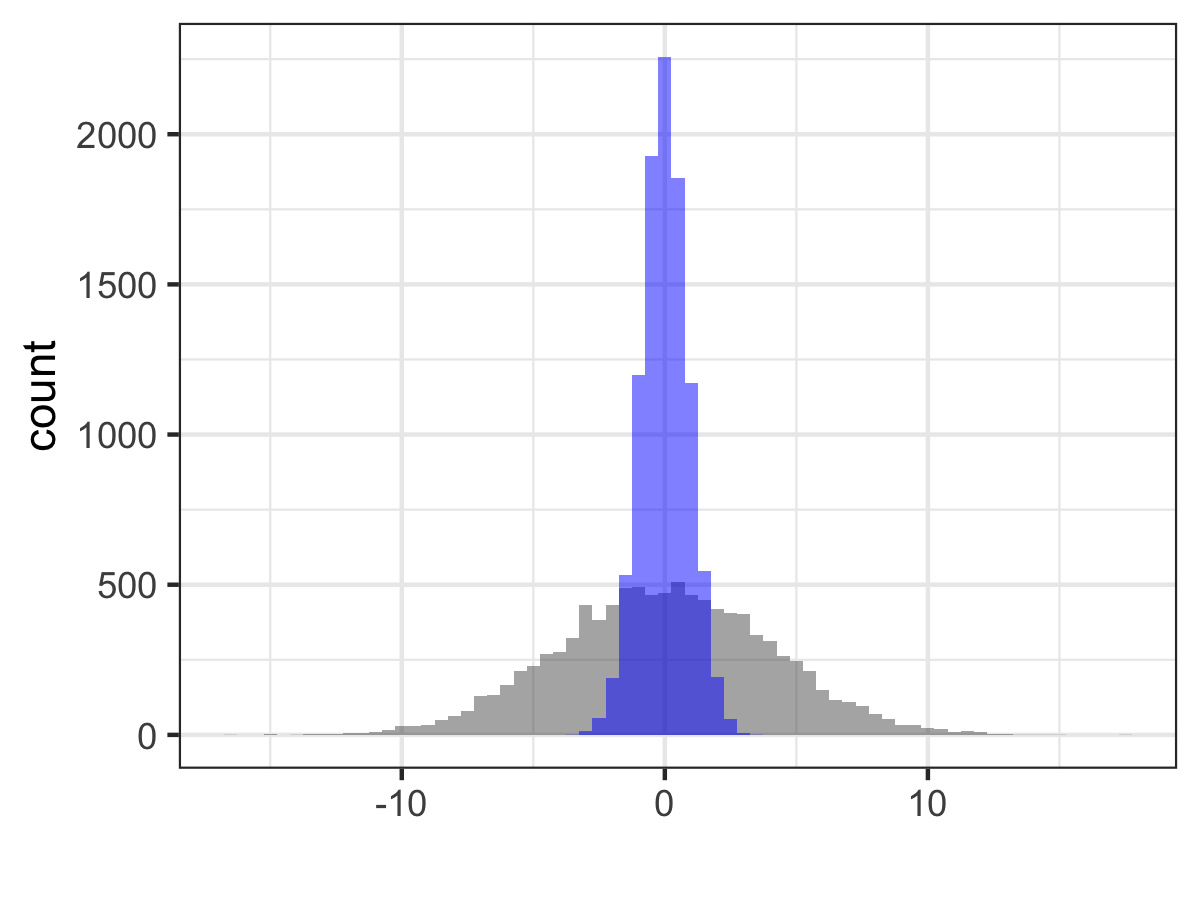
\includegraphics[width=\textwidth]{img/hyp-norm-mean.png}
    \end{subfigure}
    \begin{subfigure}{0.4\textwidth}
    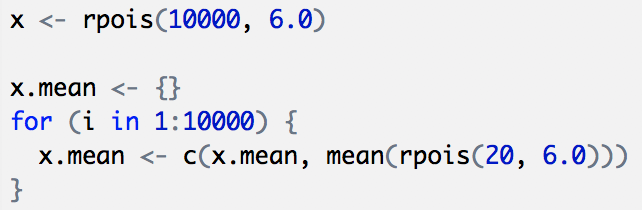
\includegraphics[width=\textwidth]{img/clt-rpois-code.png}
    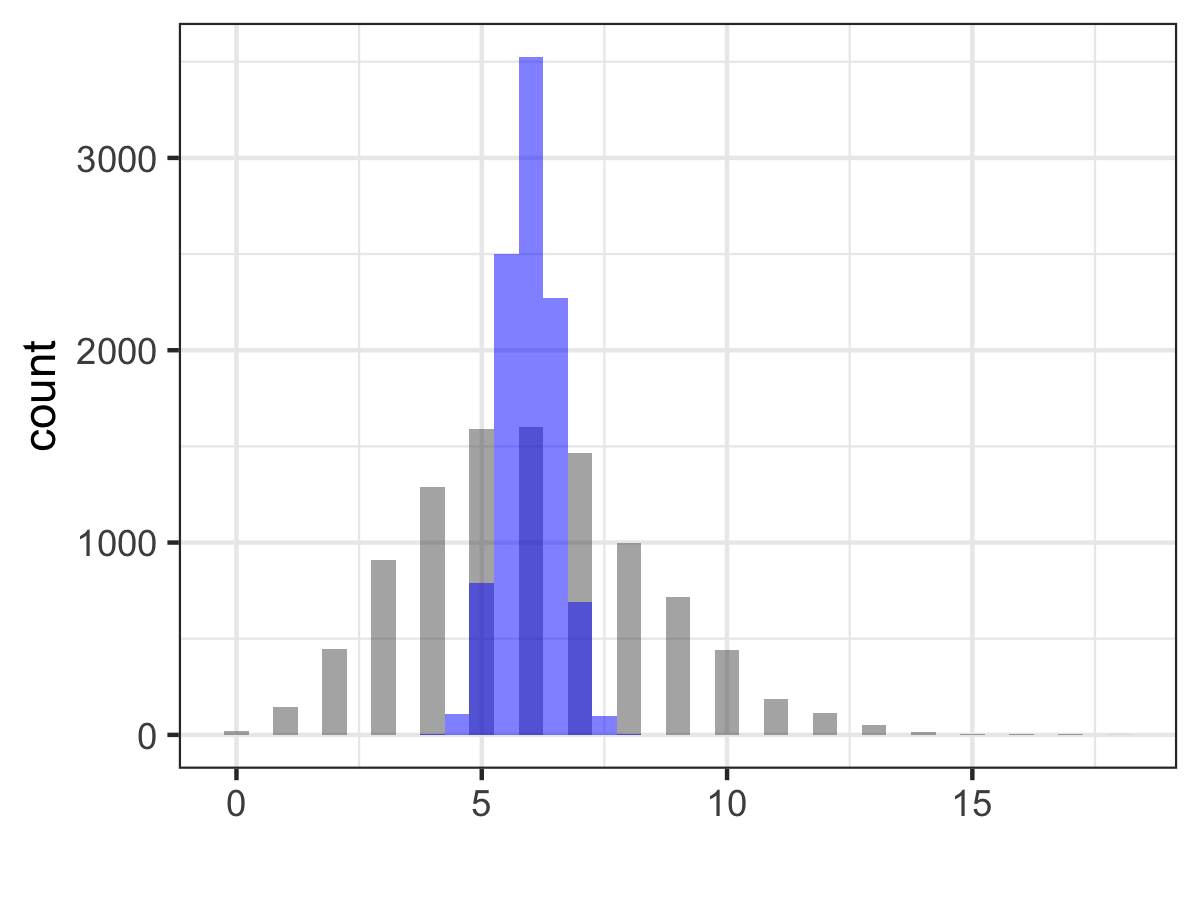
\includegraphics[width=\textwidth]{img/hyp-pois-mean.png}
    \end{subfigure}
    \begin{subfigure}{0.4\textwidth}
    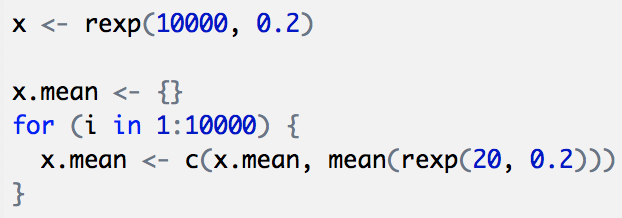
\includegraphics[width=\textwidth]{img/clt-rexp-code.png}
    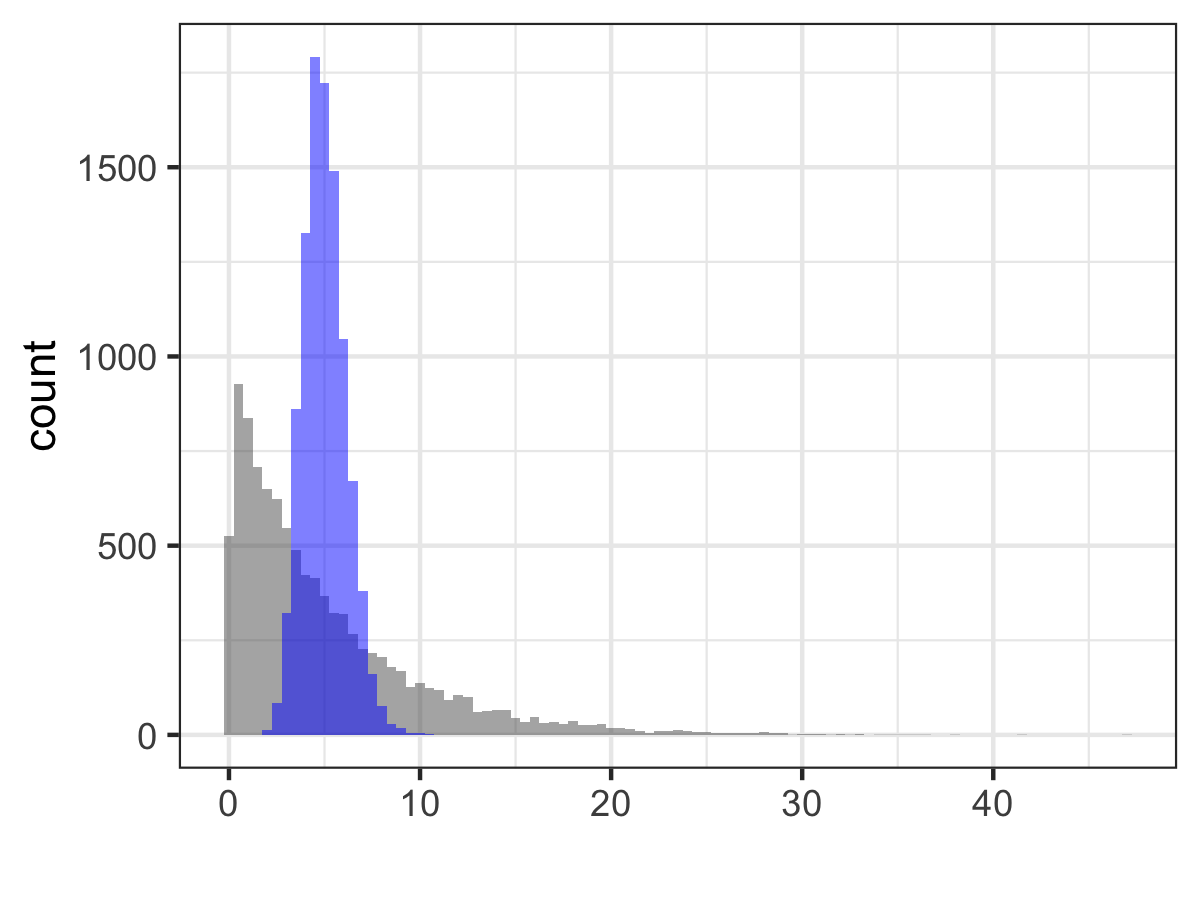
\includegraphics[width=\textwidth]{img/hyp-exp-mean.png}
    \end{subfigure}
    \begin{subfigure}{0.4\textwidth}
    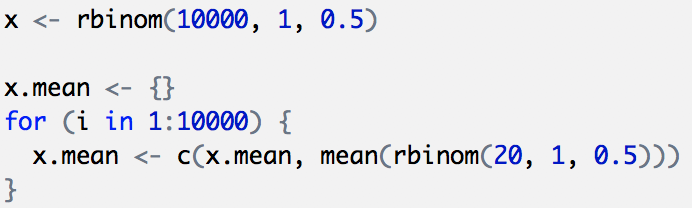
\includegraphics[width=\textwidth]{img/clt-binom-code.png}
    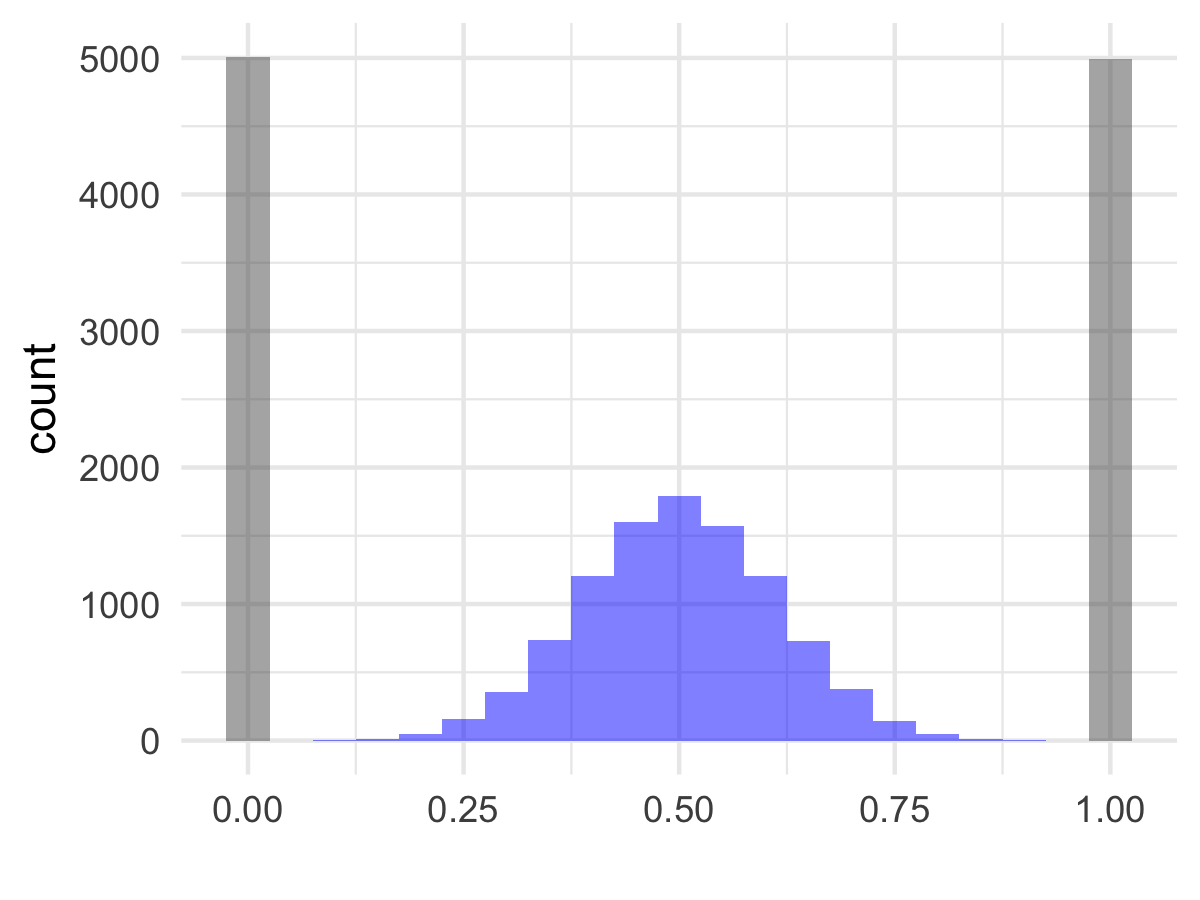
\includegraphics[width=\textwidth]{img/hyp-sum-mean.png}
    \end{subfigure}
\end{center}
\end{figure}